%% LaTeX2e class for student theses
%% sections/evaluation.tex
%% 
%% Karlsruhe Institute of Technology
%% Institute for Program Structures and Data Organization
%% Chair for Software Design and Quality (SDQ)
%%
%% Dr.-Ing. Erik Burger
%% burger@kit.edu
%%
%% Version 1.3.3, 2018-04-17

\chapter{Modellierung}
\label{ch:modellierung}
Im Folgenden soll zunaechst untersucht werden ob und wie eine konkrete MOM in Palladio modelliert werden kann und an welchen Stellen die Modellierung an ihre Grenzen kommt. Im Anschluss werden Ansätze vorgestellt, mit denen diese Probleme versucht wurden zu beheben.

%Warum sinnvoll eine MOM explizit zu modellieren? \\
%- eroeffnet neue Moeglichkeiten \\
%- bestimmte effekte mit bisheriger modellierung nicht moeglich\\
\section{Anforderungserhebung}
Aus Definition von MOMs (siehe Grundlagen) und den Messungen aus (siehe Benchmarks) wurden Anforderungen an eine Modellierung spezifiziert. \\
Was soll eine MOm koenen?\\
Asynchron Nachricht senden \\
Asynchron Nachricht empfangen \\
bestimmte Topics/Queues\\
Eingaben durch benutzer: \\
Groesse der Nachrichten angeben (siehe Benchmarks einfluss auf Latenz)\\
Anzahl der Nachrichten angeben \\
Angabe des Durchsatzes \\
Ausgabe: \\
Queue verhalten \\
Antwortzeit/Latenz der Nachrichten \\

Wie bereits in Grundlagen beschrieben gibt es fuer PCM die moeglichkeit eine MOM zu modellieren (Integration Event Based Communication)\\
- Problem:  \\
-- Kommunikation nur in eine Richtung \\
-- kein abholen von Nachrichten moeglich \\
-- kein Modellieren von Queues moeglich (aquire/release \\
-- nur RDs in verschiedenen Verarbeitungsschritten angeben auf dem Weg zum Ziel \\
Im Folgenden soll beschrieben werden, wie ein Modell aussehen soll, das eine MOM abbildet und die Anforderungen erfüllt. \\

Das Ziel ist es eine allgemeine MOM Modellierung zu erstellen, die das Verhalten einer MOM abbilden kann. Dabei soll nicht Wert auf ein spezielles Verhalten gelegt werden. Stattdessen soll es moeglich sein die Modellierung um Konfigurationen, wie zum Beispiel RMQs lazy Queues, erweitern zu koennen. 

\section{Modell}
Ziel: Modellierung mit bestehenden Elementen.\\
Anhand der bekannten MOM Architekturen aus der Untersuchung verschiedener MOMs wurde versucht zu definieren wie eine MOM modelliert werden kann. Dabei wurden die Anforderungen versucht umzusetzen. \\
- 2 Moeglichkeiten entweder mit oder ohne Exchange explizit zu modellieren.\\
- Vorteil Explizit: RDs fuer verteilung (konnte aber nicht ausgemessen werden) \\
- Nachrichten Typen mitschicken (fanout, direct) und in Branches auswerten

\subsection{Repository}
Die untersuchten Architekturen hatten als Gemeinsamkeit einen Verteiler (Exchange) und eine Warteschlange. \\

Modellierung von einem Exchange als BC und einer Queue als BC mit passiver Ressource \autoref{img:mom_repository} \\

Exchange verteilt Msgs\\

Queues wurden als Passive Ressource modelliert. Ein Aquire wurde als Consume und ein Release als Produce interpretiert. Dieser Ansatz ermöglicht es jedoch nicht einzelne Nachrichten durch das System zu verfolgen. \\

Exchange required eine Queue. a ein exchange mehrere Queues haben kann muss ein Exchange auch mehrere Queues requiren. Ausserdem muss er entscheiden koennen an welche Queue er senden oder von welcher er nachrichten empfaengt. Dies soll mithilfe von guarded branches gemacht werden. Fuer jede angeschlossene Queue gibt es einen branch. Nachricht hat bytesize und nen Type anhand dessen sie in eine Queue kommt. Oder Empfaenger sagt, wie viel Byte er aus einer bestimmten Queue heraus nehmen moechte. \\

\begin{figure}
\center
  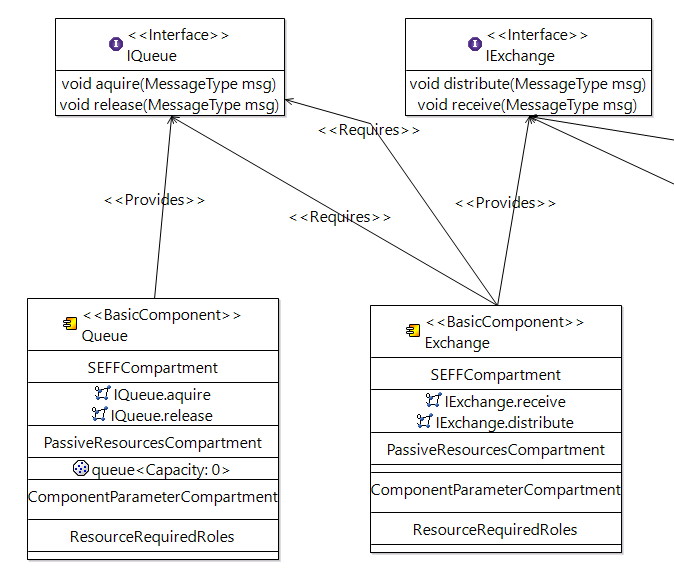
\includegraphics[width=1\textwidth]{images/mom_repository.png}
  \caption{Anwendungszenario des SpecJms}
  \label{img:mom_repository}
\end{figure}

\subsection{System}
Im System werden Queues mit dem Exchange \autoref{img:mom_system}\\
Sender und Empfaenger werden jeweils an den Exchange angeschlossen. Fuer Senden und Empfangen jeweils eine Porivided Role.

\begin{figure}
\center
  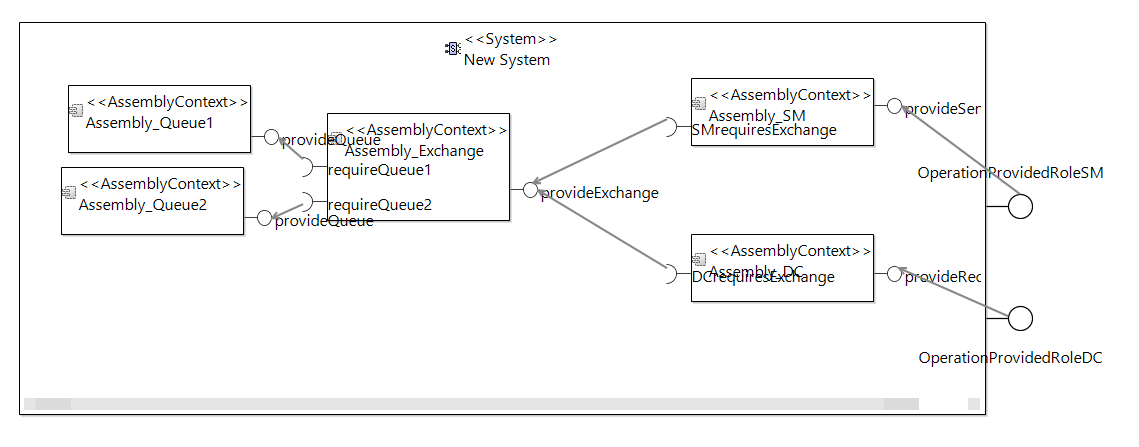
\includegraphics[width=1\textwidth]{images/mom_system.png}
  \caption{Anwendungszenario des SpecJms}
  \label{img:mom_system}
\end{figure}

\subsection{Usage}
Benutzer gibt an ob er empfangen oder senden will. \\
Benutzer gibt an welche Queue/Topic er wie viel Byte senden/empfangen moechte. \\
Ankunftsrate als Hebel um Sende-Empfangrate abzubilden \\
\subsection{Ressource Environment und Allokation}
Einen Server fuer Exchange \\
Jede Queue kann auf anderer Ressource deployed sein. die am Ende mit dem Exchange Server verbunden sein muss.\\
Fuer LR kann RD angegeben werden.

\section{Ressource Demands}
Fuer RDs wurden die Messungen aus (Benchmarks) herangezogen. \\ 
Das Ziel ist, dass der Benutzer keinen MOM spezifischen RD angeben muss. \\
In \autoref{sec:maxthroughput} wurde gemessen, was die moegliche Datenmenge ist, die gesendet werden kann (Durchsatz). Dieser Wert wird im Ressource Environment in die jeweiligen Linking Ressources eingetragen. Dabei wird fuer den LR zwischen Sender und MOM der Wert fuer keine Empfaenger eingetragen und fuer die LR zwischen Empfaenger und MOM der Wert fuer mit Empfaenger. \\

Latenz einer Nachricht mit verschiedener Bytegroesse wurde ausgemessen (siehe latenz verschiedenen Msg größen). Mithilfe einer Regressionsanalyse konnte ein RD der Form (7 * (msg.BYTESIZE + 110588)) / 489 identifiziert werden.\\

Wo Nachrichten hingeschrieben wurden waren auch ein wichtiger Einflussfaktor. Deshalb wurde fuer RMQ fuer den Fall das Lazy Queues simuliert werden sollen ein RD der Form:... aus der Differenz der Messungen mit und ohne LazyQueues bestimmt. \\

Falls die Netzwerklatenz betrachtet werden soll, kann diese in der jeweiligen LR eingetragen werden.\\

Als Eingabe fuer das System soll im Usage Modell die zu sendende Nachrichtengroesse mithilfe einer UsageVariable und der Characteristic: Bytesize angegeben werden.\\

Die Anzahl an Nachrichten die gesendet oder empfangen werden koennen werden ueber die Ankuftzeit gesteuert.\\
ArrivalTime / Anzahl Msgs \\
oder einfach BYTESIZE = Bytesize * Anazahl Nachrichten \\

- TODO: tabelle mit Werten fuer alle RDs\\

Somit sollte sich fuer die Response Time folgendes ergeben: Response Time: ByteSize / Throughput + RD / CPU + Latency + HddRD/HDD \\
%RD an Aquire um Latenz abzubilden

%Als erstes sollte die Sende und Empfangsrate abgebildet werden. Beobachtet man (ref zu Messung verschiedene Senderaten) bemerkt man fuer die ersten Messungen, solange Warteschlange nicht allzu voll wird, einen linearen Anstieg der Latenz. Daraus laesst sich zunaechst folgender RD ableiten:






%Latenz: Unter Latenz versteht man im MOM Kontext, die Zeit, die eine einzelne Nachricht braucht um beim Consumer anzukommen. Da jede Nachricht einen Zeitstempel bekommt kann die Zeit gemessen werden, wenn sie aus der Warteschlange entnommen wurde.

%welche Effekte koennen wir so hoffentlich abbilden

\section{Untersuchung des MOM Bausteins}
Uerberpruefe ob die Simulation des Modells mit Benchmark Messung passen.\\

Einfaches Szenario: Sender/Empfaenger, einer sendet, einer empfaengt.\\



Simulation 1: \\
Ankunftszeiten gleich \\
Bytesize sind zwische 100 und 10000 \\
Queue sollte immer leer sein, weil Nachricht gleich raus genommen \\
Vergleich mit echten Messungen \\
- RespnseTime \\
- Queue verhalten \\

Simulation 2: \\
- Simulation 1, aber diesmal mit Latenz (bei Linking Ressouce)\\

Simulation 3: \\
- unterschiedliche Ankuftszeiten Sender 0.5 und Empfaenger 1 \\
-> Ansteigen der Queue \\

Simulation 4: \\
Wie simulation 3, aber jetzt weiterer Empfaenger mit gleicher Ankunftszeit \\
-> Queue wieder leer\\

Simulation 5: \\
- Max Durchsatz \\
- eine Nachricht mit max Bytesize schicken \\
-> Response time sollte kontinuirlich ansteigen \\


Simulation 6: \\
- lazyqueues \\
- HDD RD hinzufuegen \\
-> Response time sollte ansteigen \\



%Die Nachrichtenmenge sollen ueber die Ankunftsrate des Senders und Empfaengers geregelt werden. Die Idee ist, dass es keinen Unterschied macht ob ein sender pro Zeiteinheit 1000 Nachrichten verschickt oder pro Zeiteinheit 1000 mal Ankommt und jeweils eine Nachricht verschickt. Sommit erhalten wir fuer Sende- und Empfangsrate die Formel: 1 / Senderate.



\section{Grenzen}
Dieser Ansatz ermöglicht es jedoch nicht einzelne Nachrichten durch das System zu verfolgen\\

welche Moeglichkeiten gibt es? Dominiks Queue Modell. Direkt drauf verweisen, oder eine/diese Idee beschreiben.\\
%Queue Fuellstand ist unbekannt \\

%Nachdem eine MOM in das Experimentsystem eingebaut wurde, soll sie im Anschluss in Palladio modelliert werden. Wie bereits erwähnt existiert eine Palladio Modellierung des Experimentsystem, auf der aufgebaut werden kann. Bei der Modellierung der MOM soll zunächst die Standardkonfiguration und in späteren Iterationen Parametrisierbarkeit modelliert werden. Dazu soll zunächst versucht werden die MOM mithilfe vorhandener PCM Elementen zu modellieren und Unzugänglichkeiten zu identifizieren. Die Idee ist, mithilfe von Architecture-Templates \cite{architcturetemplate} diese Unzugänglichkeiten zu beseitigen. Dabei handelt es sich um wiederverwendbare Muster, die auf Palladio-Modelle angewendet werden können. Beispielsweise kann anstelle der manuellen Modellierung eines Lastverteilers auch das Architectural-Template für Lastverteiler verwendet werden. %Da diese Anwendung nur aus wenigen kleinen Schritten besteht, können Architekten viel Modellierungsaufwand einsparen.


%(-- RabitMQ Config:)\\% https://www.rabbitmq.com/configure.html\\
%(-- Kafka Config:)\\ %https://kafka.apache.org/documentation/#brokerconfigs 

